\documentclass[a4paper,oneside]{scrartcl} %twocolumn,
\usepackage[utf8]{inputenc} %für MAC: applemac; für Windows: latin1 statt utf8
\usepackage[T1]{fontenc}
\usepackage[ngerman]{babel}

\usepackage{amsmath}
\usepackage{amsfonts}
\usepackage{amssymb}

\usepackage{mathptmx}
\usepackage{microtype}
\usepackage[nice]{nicefrac}

\usepackage{booktabs}
\usepackage{graphicx}
\usepackage{float}
\usepackage{hyperref}
\usepackage{wrapfig}


\setkomafont{captionlabel}{\upshape\bfseries}
\setkomafont{caption}{\itshape}


\title{Rastertunnelmikroskop}
\author{Robi Pedersen \and Simon Schmeißer}
\date{Versuchsdurchführung 16.09. - 17.09.2010}

\hypersetup{pdftitle={Rastertunnelmikroskop},
	    pdfauthor={Robi Pedersen, Simon Schmeißer}}

\providecommand{\e}[1]{\ensuremath{\times 10^{#1}}}

\providecommand{\bild}[2]{\begin{figure}[H]
				\centering \includegraphics*[viewport= 5 225 322 520 , width = 0.6\textwidth]{messwerte/#1}
				\caption{#2} 
				\end{figure} }

\providecommand{\parameter}[3]{\begin{center}
				\begin{tabular}[H]{l c}
				Image Width & #1 nm\\ Time/Line & #2 s\\ Points/Line & #3\\
				\end{tabular}
				\end{center} }

\providecommand{\zweid}[4]{\begin{figure}[H]
				\begin{minipage}{0.5\textwidth}
				\centering \includegraphics*[viewport= 5 528 322 825 , width = \textwidth]{messwerte/#1}
				\caption{#2}
				\end{minipage}
				\begin{minipage}{0.5\textwidth}
				\centering \includegraphics*[viewport= 5 528 322 825 , width = \textwidth]{messwerte/#3}
				\caption{#4}
				\end{minipage}
				\end{figure} }

\providecommand{\zweiunddreid}[1]{\begin{figure}[H]
				    \begin{minipage}{0.5\textwidth}
				    \centering \includegraphics*[viewport= 5 528 322 825 , width = \textwidth]{messwerte/#1}
				    \end{minipage}
				    \begin{minipage}{0.5\textwidth}
				    \centering \includegraphics*[viewport= 5 5 322 300 , width = \textwidth]{messwerte/#1}	
				    \end{minipage}
				    \end{figure} }

\providecommand{\bildmitdesc}[4]{\begin{center}
				\begin{tabular}[H]{l l l c}
				#1 & & Image Width & #2 nm\\ & & Time/Line & #3 s\\ & & Points/Line & #4\\
				\end{tabular}
				\end{center}}

\providecommand{\bildmitdescpic}[5]{\begin{center}
				\begin{minipage}{0.6\textwidth}
				\begin{tabular}[H]{l l l c}
				#1 & & Image Width & #2 nm\\
				   & & Time/Line & #3 s\\
				   & & Points/Line & #4\\
				\end{tabular}
				\end{minipage}
				\begin{minipage}{0.25\textwidth}
				    \includegraphics*[viewport= 5 528 322 825 , width = 0.8\textwidth]{messwerte/#5} \\
				\end{minipage}
				\end{center}}

\providecommand{\bildmitdescpicnureinbild}[5]{\begin{center}
				\begin{minipage}{0.6\textwidth}
				\begin{tabular}[H]{l l l c}
				#1 & & Image Width & #2 nm\\
				   & & Time/Line & #3 s\\
				   & & Points/Line & #4\\
				\end{tabular}
				\end{minipage}
				\begin{minipage}{0.25\textwidth}
				    \includegraphics*[viewport= 5 225 322 520 , width = 0.8\textwidth]{messwerte/#5} \\
				\end{minipage}
				\end{center}}

\begin{document}
\begin{titlepage}
  \maketitle
  \vfill
  \thispagestyle{empty}
\end{titlepage}

\tableofcontents
\clearpage
%*****************************************************************

\section{Aufgabenstellung}

\begin{enumerate}

\item Pockelseffekt: Für eine Pockelszelle bestimme man die Halbwellenspannung $U_{\lambda/2}$ und berechne daraus den elektrooptischen Koeffizienten $r_{41}$, indem man
\begin{enumerate}
	\item eine Spannung in Sägezahnform
	\item eine sinusmodulierte Gleichspannung
\end{enumerate}
an die Zelle anlegt.

\item  Faraday-Effekt: Für einen in einer stromdurchflossenen Spule befindlichen Schwerflintstab bestimme man die Verdet-Konstane mit Hilfe eines Halbschattenpolarimeters.

\end{enumerate}
\section{Theoretische Grundlagen}

\subsection{Kernspin}

Neben den Elektronen, besitzen auch die Protonen und Neutronen einen Spin, einen intrinsischen, diskreten Drehimpuls $\vec I$. Dieser ist gegeben durch:

$$ |\vec I| = \hbar \sqrt{I(I+1)} $$

In z-Richtung (in unserem Fall auch die Richtung des Feldes des Permanentmagneten) kann der Spin auch nur ganzzahlige Vielfache von $\hbar$ annehmen, nämlich

$$I_z = \hbar\cdot m_I$$

wobei $m_I$ die magnetische Spinquantenzahl ist und nur ganzzahlige Werte zwischen $-I$ und $I$ annehmen kann. Es gibt also $2I+1$ verschiedene Spinzustände. Bei Fermionen ist $I=1/2$ und daher $m_I = \pm\frac{1}{2}$, es gibt also zwei verschiedene Spineinstellungsmöglichkeiten für ein Energieniveau.

\subsubsection{Magnetisches Moment}

Da der Spin als Eigendrehimpuls eines Teilchens aufgefasst werden kann, induziert ein Teilchen mit Spin und einer Ladung ein magnetisches Dipolmoment, welches durch das gyromagnetische Verhältnis $\gamma$ direkt mit dem Spin zusammenhängt. (Wir erläutern hier nur die spezifischen Formeln für den Kernspin des Protons).

\begin{equation} \vec \mu_I = \gamma\cdot\vec I = \frac{g_K\cdot\mu_K}{\hbar}\vec I \label{gyro}\end{equation}

$\mu_K$ ist hier das Kernmagneton und ist eine Konstante:

$$\mu_K = \frac{e\cdot \hbar}{2\cdot m_p} \approx 3.15\e{-8} eV/T$$

und $m_p$ ist die Masse des Protons. In z-Richtung gilt somit für das magnetische Moment:

\begin{equation} \mu_z = g_K \cdot \mu_K \cdot m_I \label{muz} \end{equation}

\subsubsection{Spin im Magnetfeld}

Die potentielle Energie eines magnetischen Moments in einem Magnetfeld $\vec B$ ist gegeben durch:

$$ E_p = -\vec\mu\cdot\vec B $$

Legt man das $\vec B$-Feld o.B.d.A in z-Richtung, so erhält man folgenden Zusammenhang:

$$ E_p = -\mu_z\cdot B_z \stackrel{(\ref{muz})}{=} -g_K \cdot \mu_K \cdot m_I\cdot B_z $$

Die Energie eines spinbesetzten Teilchens in einem $\vec B$-Feld hängt also von der Stärke des $\vec B$-Felds ab und von dessen magnetischen Spinquantenzahl, also seinem Spin-Zustand. Spin-up-Teilchen ($m_I = +1/2$) haben also eine andere Energie als Spin-down-Teilchen ($m_I = -1/2$). Dies bezeichnet man als Zeeman-Aufspaltung der Spinzustände. Der Energieunterschied zwischen eines Spin-up- und eines Spin-down-Teilchens ergibt sich also durch:

\begin{equation} \Delta E = E_p(\uparrow) - E_p(\downarrow) =  g_K \cdot \mu_K \cdot B_z \label{de} \end{equation}

Diese Energie muss aufgebracht werden um einen Spin-down in einem Magnetfeld in ein Spin-up "`umzuklappen"'. Sie führt ebenfalls zur stimulierten Emission und somit zum Übergang eines Spin-up in ein Spin-down.

\subsection{Kernspinresonanz}

Die Energie aus (\ref{de}) kann man natürlich auch mit elektromagnetischer Strahlung erreichen. Hat die Strahlung genau die richtige Frequenz, die sogenannte Resonanzfrequenz $\nu_r$, so kann sie Spin-Übergänge induzieren. In diesem Fall gilt:

$$ \Delta E = E_\nu \ \Leftrightarrow \ g_K \cdot \mu_K \cdot B_z = h\cdot \nu_r $$

Die Resonanzfrequenz ist also gegeben durch:

\begin{equation} \nu_r = \frac{g_K \cdot \mu_K \cdot B_z}{h} \label{g} \end{equation}

Man spricht in diesem Fall von Kernspinresonanz. 

\subsubsection{Zustandsbesetzung}

Die induzierten Übergänge passieren anhand von Absorption und stimulierter Emission der Photonen. Die Wahrscheinlichkeit für Absorption oder Emission ist abhängig von der Anzahl der Teilchen im tieferen ($N_{tief}$)bzw. im höheren ($N_{hoch}$) energetischen Zustand. Im thermischen Gleichgewicht unterliegen die Teilchen einer Boltzmann-Verteilung:

$$\frac{N_{hoch}}{N_{tief}} = \exp(-g_K\cdot\mu_K\cdot B_z/k_B\cdot T)$$

Würden wir die Zahlenwerte unseres Experiments einsetzen erhielten wir einen Besetzungsunterschied von etwa $3\e{-6}$, was etwa $10^{17}$ Teilchen entspricht.

Durch resonante Anregung ergäbe sich ein neues dynamisches Gleichgewicht, bei dem das Verhältnis der Zustände gerade so eingestellt ist, dass die Übergangswahrscheinlichkeiten gleich groß sind. 

\subsubsection{Relaxation}

Das System würde also die erwartete resultierende Absorption zeigen, bis es sich in einem Gleichgewicht befinden würde. Jedoch spielen noch andere wesentliche Vorgänge eine Rolle, am wichtigsten die Spin-Gitter-Relaxation:
Die Energie eines Spinübergangs kann nämlich auch strahlungslos erfolgen, indem sie an ein Phonon abgegeben wird und somit Gitterschwingungen anregt und Wärme verursacht, so dass die Verteilung entsprechend der Boltzmann-Statistik wiederhergestellt wird.
Als anderen Relaxationsprozess gibt es noch die Spin-Spin-Relaxation, die den Effekt beschreibt, dass Spins miteinander wechselwirken und somit die Absorptionslinie verbreitern. 
Durch Zusatz von paramagnetischen Ionen können diese Relaxationszeiten um Größenordnungen verkürzt werden. In unserem Fall handelt es sich dabei um $Mn(NO_3)_2 + 4 H_2O$
Diese Relaxationsprozesse werden auch als transversale (Spin-Spin-WW) und longitudinale (Spin-Gitter-WW) Relaxation bezeichnet.

\subsection{Hall-Sonde}

Eine Hall-Sonde nutzt den Hall-Effekt zur Messung von magnetischen Feldstärken. Wird sie von Strom durchflossen und in ein Magnetfeld gebracht, so werden die Elektronen durch die Lorentz-Kraft senkrecht zu diesen beiden Feldern im Leiter bewegt. An einer Stelle im Leiter entsteht also ein Überschuss an Elektronen, während auf der anderen Seite ein Mangel entsteht. Diese Ladungsverteilung induziert ein elektrisches Feld, dessen Kraft der Lorentz-Kraft entgegenwirkt, bis ein Gleichgewicht eintritt. Diese Spannung wird nun gemessen und ist direkt proportional zum Magnetfeld, so dass sich dieses durch einen Umrechnungsfaktor bestimmen lässt.

\subsection{Das Lock-In Verfahren}

Das Lock-In-Verfahren ist ein Messverfahren, welches den Vorteil hat, dass ein Nutzsignal aus großen Störungen heraus gefiltert werden kann. Dazu wird das Signal mit einer festen Frequenz getaktet, die auch an den Verstärker als Referenzsignal weitergegeben wird, so dass dieser nur empfindlich auf Signale genau dieser Frequenz ist.
In unserem Fall modulieren wir das Magnetfeld mit einer Sägezahnfunktion, die wiederum von einem Sinus moduliert wird. In der Nähe der Resonanz wird diese im Sinustakt überstrichen und das Absorptionssignal dementsprechend getaktet.

\section{Versuchsbeschreibung}



\section{Durchführung}


Wir haben den PC hochgefahren und dann das Messprogramm \emph{Nanosurf easyscan 2} gestartet. Dann haben wir eine Spitze anhand einer Kneifzange aus dem $PtIr$-Draht hergestellt und mit einer Pinzette in das Rastertunnelmikroskop eingeführt. Unsere erste Messung haben wir mit Graphit durchgeführt. Wir haben bei jeder Messung die Spitze grob an die Probe herangefahren. 

In diesem Fall haben wir für die feinere Annäherung wir folgende Schritte durchgeführt:



\begin{table}[H]
\caption{Graphit\_1.png}
\centering \begin{tabular}[H]{l c c l}
Funktion & Approach Speed & Tip Voltage & Resultat/Bemerkung\\ \hline
Approach & 52\% & 0.15 V & grün-rot blinkend\\
Withdraw & & & orange\\
Approach & 29\% & 0.15 V & grün\\
 & 21\% & 90 mV & grün\\
 & 20\% & 50 mV & grün\\
\end{tabular}
\end{table}


Wir haben dann ein Bild aufgenommen mit folgenden Parametern:

\parameter{1.5}{0.4}{256}

\bild{Graphit_1}{Graphit\_1.png}

Nach diesem ziemlich verfehlten Bild haben wir eine neue Spitze hergestellt und eingesetzt. Wir haben eine erneute Messung des Graphits durchgeführt: 

\begin{table}[H]
\caption{Graphit\_2.png}
\centering \begin{tabular}[H]{l c c l}
Funktion & Approach Speed & Tip Voltage & Resultat/Bemerkung\\ \hline
Approach & 50\% & 0.15 V & orange\\
 & 40\% & 0.15 V & rot\\
Retract & & & orange\\
Approach & 25\% & 0.15 V & orange\\
 & 20\% & 0.15 V & orange - abgebrochen\\
 & 27\% & 0.15 V & orange\\
 & 24\% & 0.15 V & orange\\
 & 23\% & 90 mV & orange - abgebrochen\\
 & 25\% & 90 mV & grün\\
 & 20\% & 50 mV & grün\\
 & 20\% & 25 mV & grün\\
\end{tabular}
\end{table}

Wir haben immer dann abgebrochen, wenn das Heranfahren der Nadel viel zu lange gedauert hat, also deutlich einige Minuten überschritten hat. Wir haben das Bild \emph{Graphit\_2.png} mit folgenden Parametern aufgenommen: 

\parameter{1.5}{0.4}{256}

In der Auswertung kann man alle relevanten Bilder einsehen. Wir beschreiben hier nur wie wir vorgegangen sind, um die Bilder aufzunehmen. Die Namen der Bilder entsprechen den angegebenen Namen über den Tabellen.

Wir haben in das Bild \emph{Graphit\_2.png} hineingezoomt und nach dem Feineinstellen nochmal eine genauere Messung durchgeführt. (x-Position = -1.3 nm , y-Position = -42 nm). Wir mussten hier nochmal die Nadel neu heranführen, da die Kontrolllampe orange war. 

\begin{table}[H]
\caption{Graphitmessung}
\centering \begin{tabular}[H]{l c c l}
Funktion & Approach Speed & Tip Voltage & Resultat/Bemerkung\\ \hline 
Approach & 46\% & 25 mV & rot\\
Withdraw & & & orange\\
Approach & 35\% & 25 mV & grün\\
\end{tabular}
\end{table}

\parameter{1.5}{0.8}{512}

An dieser Stelle haben wir wieder eine neue Spitze gemacht, da dieses Bild wieder sehr unklar war, was vielleicht daran liegen kann, dass wir beim ersten Approach die Probe mit der Spitze berührt haben (rote Kontrollleuchte), und somit vielleicht die Spitze deformiert haben. Wir haben es nochmal versucht:

\begin{table}[H]
\caption{Graphitmessung}
\centering \begin{tabular}[H]{l c c l} 
Funktion & Approach Speed & Tip Voltage & Resultat/Bemerkung\\ \hline
Approach & 46\% & 25 mV & rot\\
Withdraw & & & orange\\
Approach & 35\% & 25 mV & grün\\
\end{tabular}
\end{table}

\parameter{1.5}{0.6}{512}

und nochmal mit neuer Spitze:

\begin{table}[H]
\caption{Graphitmessung}
\centering \begin{tabular}[H]{l c c l} 
Funktion & Approach Speed & Tip Voltage & Resultat/Bemerkung\\ \hline
Approach & 40\% & 0.1 V & rot\\
Withdraw & & & orange\\
Approach & 30\% & 0.1 V & grün\\
 & 20\% & 25 mV & grün\\
\end{tabular}
\end{table}

\parameter{5.58}{0.6}{256}

Da alle diese Bilder ziemlich nutzlos waren sind wir an dieser Stelle aus frustrationstechnischen Gründen auf eine andere Probe umgestiegen, nämlich das 160-nm-Gitter (\emph{Nano-Grid}) und haben wiederum eine neue Spitze angefertigt. Das Heranführen der Nadel war jedoch erfolglos, da das Rastertunnelmikroskop keinen Tunnelstrom registrieren konnte. Wir haben somit unsere Messungen mit Molybdändisulfid fortgeführt.

\begin{table}[H]
\caption{MoS2\_1.png, MoS2\_2.png, MoS2\_3.png}
\centering \begin{tabular}[H]{l c c l} 
Funktion & Approach Speed & Tip Voltage & Resultat/Bemerkung\\ \hline
Approach & 50\% & 0.15 V & rot\\
Withdraw & & & orange\\
Approach & 30\% & 0.15 V & rot\\
Withdraw & & & orange\\
Approach & 20\% & 25 mV & grün\\
 & 20\% & 0.90 V & grün\\
\end{tabular}
\end{table}

Wir haben 3 Bilder mit jeweils verschiedenen Zooms bei dieser Einstellung gemacht. Die Bildparameter lauten:

MoS2\_1.png \parameter{351.4}{0.4}{128}
MoS2\_2.png, \ \ \ Zoom: x-Pos = -17 nm , y-Pos = -0.17 nm \parameter{37.06}{0.4}{128}
MoS2\_3.png, \ \ \ Zoom: x-Pos = -16 nm , y-Pos = -0.17 nm \parameter{12.31}{0.4}{128}

Nach einem erneuten vergeblichen Versuch, das Nano-Grid zu messen, haben wir eine weitere Messung des $MoS_2$ gemacht. Der Approach lief folgendermaßen ab:

\begin{table}[H]
\caption{Molybdändisulfidmessung}
\centering \begin{tabular}[H]{l c c l} 
Funktion & Approach Speed & Tip Voltage & Resultat/Bemerkung\\ \hline
Approach & 40\% & 0.15 V & rot\\
Withdraw & & & orange\\
Approach & 25\% & 0.1 V & orange-abgebrochen\\
 & 30\% & 0.1 V & orange-abgebrochen\\
 & 40\% & 0.1 V & grün\\
\end{tabular}
\end{table}

Nachdem die Messung begonnen hatte, wurde das gesamte Bild auf einmal weiß und die Kontrollleuchte zeigte rot an. Wir haben einen neuen Approach versucht:

\begin{table}[H]
\caption{MoS2\_4.png}
\centering \begin{tabular}[H]{l c c l}
Funktion & Approach Speed & Tip Voltage & Resultat/Bemerkung\\ \hline
Approach & 30\% & 0.1 V & orange - abgebrochen\\
 & 35\% & 0.1 V & grün
\end{tabular}
\end{table}

\parameter{10.2}{0.2}{128}

Mit einer neuen Spitze haben wir wiederum die Graphit-Probe analysiert:

\begin{table}[H]
\caption{Graphit\_3.png}
\centering \begin{tabular}[H]{l c c l}
Funktion & Approach Speed & Tip Voltage & Resultat/Bemerkung\\ \hline
Approach & 51\% & 0.19 V & rot\\
Withdraw & & & orange\\
Approach & 35\% & 0.15 V & rot\\
Withdraw & & & orange\\
Approach& 20\% & 0.1 V & rot\\
Withdraw & & & orange\\
Approach & 39\% & 0.1 V & grün\\
\end{tabular}
\end{table}

\parameter{1.96}{0.5}{256}

Nach dem weiteren Anfertigen einer neuen Spitze, haben wir nochmal die Graphit-Probe benutzt:

\begin{table}[H]
\caption{Graphit\_4.png}
\centering \begin{tabular}[H]{l c c l}
Funktion & Approach Speed & Tip Voltage & Resultat/Bemerkung\\ \hline
Approach & 36\% & 0.15 V & grün\\
 & 30\% & 90 mV & grün\\
 & 25\% & 60 mV & grün\\
 & 20\% & 45 mV & grün
\end{tabular}
\end{table}

\parameter{2}{0.5}{128}

Wir haben wiederum eine neue Spitze angefertigt und mit der Messung des Goldes begonnen. 

\begin{table}[H]
\caption{Gold\_0, \_1, \_2, \_3.png}
\centering \begin{tabular}[H]{l c c l}
Funktion & Approach Speed & Tip Voltage & Resultat/Bemerkung\\ \hline
Approach & 31\% & 0.1 V & grün\\
 & 21\% & 45 mV & grün\\
\end{tabular}
\end{table}

Gold\_0.png \parameter{3.5}{0.5}{128}
Gold\_1.png \parameter{3.5}{0.5}{128}
Gold\_2.png \parameter{150}{0.5}{128}
Gold\_3.png \parameter{500}{0.5}{128}

Nach der Aufnahme dieser vier Bilder sind wir wieder auf die $MoS_2$-Probe umgestiegen:

\begin{table}[H]
\caption{MoS2\_5, \_6, \_7, \_8, \_9.png}
\centering \begin{tabular}[H]{l c c l}
Funktion & Approach Speed & Tip Voltage & Resultat/Bemerkung\\ \hline
Approach & 35\% & 0.15 V & orange - abgebrochen\\
 & 39\% & 0.15 V & grün\\
 & 26\% & 78 mV & grün
\end{tabular}
\end{table}

MoS2\_5.png \parameter{56.1}{0.5}{128}
MoS2\_6.png \parameter{6.13}{0.5}{128}
MoS2\_7.png \parameter{1.8}{0.5}{128}

Approach mit -36 mV und 35\% (grün)

MoS2\_8.png \parameter{1.8}{0.5}{128}

Approach mit -5.8 mV und 20\% (grün)

MoS2\_9.png \parameter{1.8}{0.5}{128}

Nach diesen Messungen haben wir eine neue Spitze gemacht und folgende Bilder mit Graphit aufgenommen:

\begin{table}[H]
\caption{Graphit\_F1, \_F2, \_F3, \_F4, \_F5.png}
\centering \begin{tabular}[H]{l c c l}
Funktion & Approach Speed & Tip Voltage & Resultat/Bemerkung\\ \hline
Approach & 44\% & 0.15 V & grün (Aufnahme von Graphit\_F1.png)\\
Approach & 31\% & 86 mV & grün (Aufnahme von Graphit\_F2.png)\\
Move & & & grün (Aufnahme von Graphit\_F3 und \_F4.png)
\end{tabular}
\end{table}

Graphit\_F1.png \parameter{5}{0.2}{128}
Graphit\_F2 und \_F3.png \parameter{5}{0.6}{256}
Graphit\_F4.png (Das Bild ist bei 2/3 des Bildes abgebrochen) \parameter{5}{1.2}{512}
Zoom in das Bild Graphit\_F4.png (x = 0.04 nm , y = 1.7 nm) \parameter{3.3}{1.2}{512}

Neuer Approach:

\begin{table}[H]
\caption{Graphit\_F6.png}
\centering \begin{tabular}[H]{l c c l}
Funktion & Approach Speed & Tip Voltage & Resultat/Bemerkung\\ \hline
Approach & 21\% & 86 mV & grün\\ 
Approach & 21\% & 51 mV & grün
\end{tabular}
\end{table}

Graphit\_F6.png: \parameter{5}{0.6}{256}

Da wir mit dieser Spitze so schöne Bilder bekommen konnten, haben wir auch gleich anhand des Messprogramms versucht, die Gitterkonstante des Graphits zu berechnen. Dazu haben wir die integrierte Längenmessfunktion benutzt. Wir haben immer mehrere Maxima gemessen und gemittelt:

\begin{center}
\begin{tabular}[H]{l c c c l}
Bild & Anzahl N & gemessene Länge L & Gitterkonstante g & Messrichtung\\ \hline
Graphit\_F4.png & 8 & 1.913 nm & 2.391 $\mathring A$ & senkrecht\\
 & 8 & 1.866 nm & 2.333 $\mathring A$ & senkrecht\\
Graphit\_F3.png & 15 & 2.954 nm & 1.970 $\mathring A$ & senkrecht\\
 & 10 & 1.974 nm & 1.974 $\mathring A$ & senktecht\\
 & 10 & 2.313 nm & 2.313 $\mathring A$ & waagerecht\\
Graphit\_F5.png & 11 & 2.059 nm & 1.872 $\mathring A$ & waagerecht\\
 & 8  & 1.873 nm & 2.341 $\mathring A$ & senkrecht\\
 & 7 & 1.627 nm & 2.324 $\mathring A$ & senkrecht
\end{tabular}
\end{center}

Die Gitterkonstante die wir in diesem Fall messen sollten ist in der Theorie 2,456 $\mathring A$. Viele unserer gemessenen Werte liegen relativ nahe an diesem Wert. Die Ausnahmen haben mit verzerrzen Bildern zu tun. Vor allem hat man bei allen Bildern verschiedene Resultate für verschiedene Messrichtungen, was auf diese Verzerrung stark hindeutet. In der Auswertung haben wir die Fehler auf diese Werte berechnet.

Wir messen nochmal das Molybdändisulfid mit dieser Spitze:

\begin{table}[H]
\caption{MoS2\_F6, \_F7, \_F8.png}
\centering \begin{tabular}[H]{l c c l}
Funktion & Approach Speed & Tip Voltage & Resultat/Bemerkung\\ \hline
Approach & 44\% & -0.15 V & grün (Messung von MoS2\_F6 und \_F7.png)\\
 & 24\% & -84 mV & grün\\
 & 24\% & -49 mV & grün (Messung von MoS2\_F8.png
\end{tabular}
\end{table}

mit den Bildparametern

MoS2\_F6.png \parameter{5}{0.2}{128}
MoS2\_F7.png \parameter{5}{0.6}{256}
MoS2\_F6.png \parameter{5}{0.6}{256}

Auch hier haben wir wieder versucht die Gitterkonstante mit dem Messprogramm zu berechnen:

\begin{center}
\begin{tabular}[H]{l c c c l}
Bild & Anzahl N & gemessene Länge L & Gitterkonstante g & Messrichtung\\ \hline
MoS2\_F7.png & 5 & 1.372 nm & 2.744 $\mathring A$ & waagerecht\\
MoS2\_F8.png & 9 & 2.430 nm & 2.700 $\mathring A$ & waagerecht\\
 & 10 & 1.724 nm & 1.724 $\mathring A$ & senkrecht\\
 & 2 & 0.4278 nm & 2.139 $\mathring A$ & senkrecht\\
\end{tabular}
\end{center}

\clearpage









\section{Durchführung und Auswertung}

\subsection{Einfluss der Einstellungen der NIM-Geräte auf das Signal}

Wir haben verschiedene Einstellungen der NIM-Geräte ausprobiert und deren Einfluss auf das Signal am Oszilloskop beobachtet. Als Signalquelle haben wir einfach die Umgebungsstrahlung genutzt und als Messgerät den Plastikszintillator.

Als erstes haben wir das Signal direkt am Vorverstärker gemessen. Danach haben wir den Einfluss der Verstärkung und der \emph{shaping time} am unipolaren Ausgang des Amplifiers auf das Signal untersucht. Schlussendlich haben wir noch den positiven Ausgang des Einkanalanalysators untersucht, indem wir die untere und die obere Schwelle eingestellt haben und die Funktion des Delays beobachtet haben.

Zusammengefasst erhielten wir folgende Signale:

\begin{figure}[H]
\begin{minipage}{0.4\textwidth}
\centering 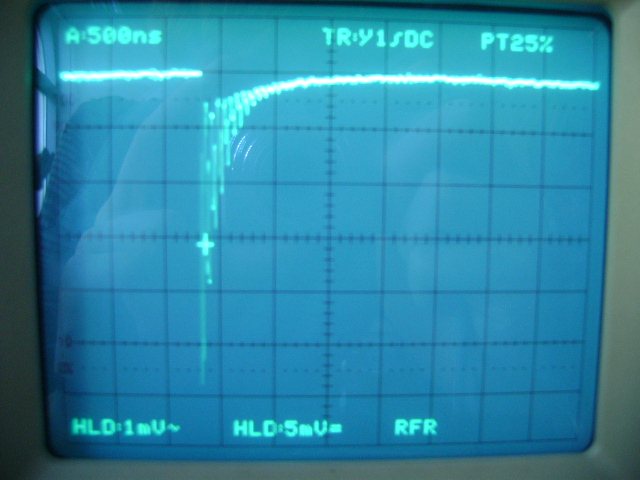
\includegraphics[width = \textwidth]{messergebnisse/1.JPG}
\end{minipage}
\begin{minipage}{0.6\textwidth}
Signal nach dem Vorverstärker.
\centering \begin{tabular}{l l}
Tiefe des Peaks & 5.8 mV\\
Breite des Peaks & 1.2 $\mu s$
\end{tabular}
\end{minipage}
\end{figure}

\begin{figure}[H]
\begin{minipage}{0.4\textwidth}
\centering 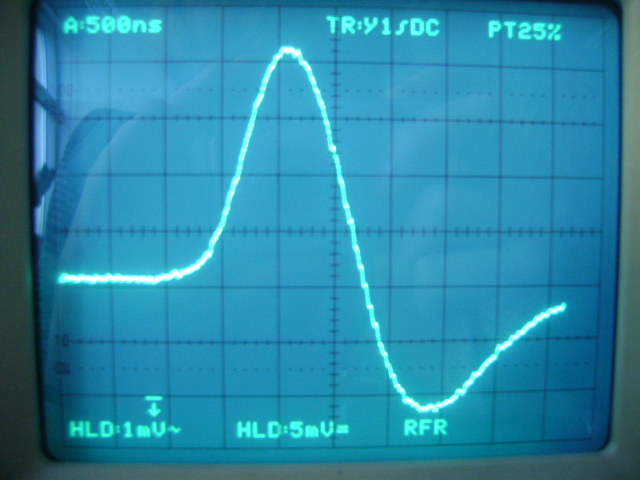
\includegraphics[width = \textwidth]{messergebnisse/2.JPG}
\end{minipage}
\begin{minipage}{0.6\textwidth}
Signal nach dem Verstärker (unipolarer Ausgang) mit einer Verstärkung von 12.6 und einer shaping time von 0.5 $\mu s$

\centering \begin{tabular}{l l}
Spannung Peak to Peak & 36 mV\\
Zeit Peak to Peak & 1.3 $\mu s$
\end{tabular}
\end{minipage}
\end{figure}

\clearpage %----------------------

Einfluss höherer Verstärkung (shaping time: 0.5 $\mu s$)
\begin{figure}[H]
\begin{minipage}{0.5\textwidth}
\centering 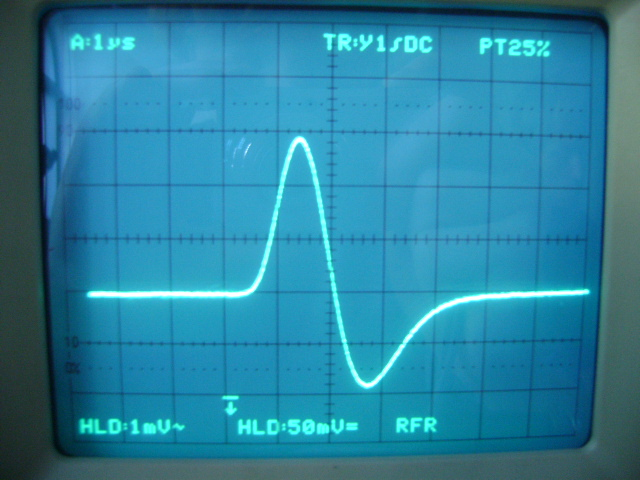
\includegraphics[width = 0.8\textwidth]{messergebnisse/3.JPG} 
\centering \begin{tabular}{l l}
Verstärkung & 100\\
Spannung Peak to Peak & 240 mV\\
Zeit Peak to Peak & 1.3 $\mu s$
\end{tabular}
\end{minipage}
\begin{minipage}{0.5\textwidth}
\centering 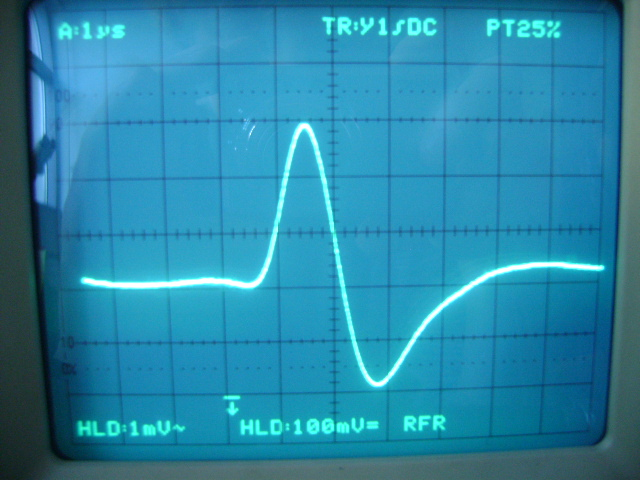
\includegraphics[width = 0.8\textwidth]{messergebnisse/4.JPG}
\centering \begin{tabular}{l l}
Verstärkung & 500\\
Spannung Peak to Peak & 580 mV\\
Zeit Peak to Peak & 1.3 $\mu s$
\end{tabular}
\end{minipage}
\end{figure}

Die Verstärkung hat also wie erwartet die Amplitude des Signals vergrößert, z.B. haben wir bei einer Einstellung der Vergrößerung von 500 das Signal bereits auf eine Amplitude von 0.6 V bringen können, wo es am Anfang gerade mal etwa 6 mV hatte (100-fache Verstärkung). 

Der Einfluss der Shaping Time auf das Signal war schwer zu beobachten, da bei größerer Shaping Time das Signal immer instabiler wurde. Wir konnten jedoch sehen, dass das Signal breiter wurde. Bei einer eingestellten Shaping Time von 1 $\mu s$ konnten wir z.B. noch messen, dass die Distanz zwischen den beiden Peaks etwa 2.3 $\mu s$ betrug, im Gegensatz zu 1.3 $\mu s$ bei einer Shaping Time von 0.5 $\mu s$. Das Verstellen der Verstärkung hatte keinen sichtbaren Einfluss auf diese Distanz.

Danach haben wir das Signal des negativen Ausgangs des Einkanalanalysators untersucht und mit dem Signal aus dem Vorverstärker verglichen.

\begin{figure}[H]
\begin{minipage}{0.4\textwidth}
\centering 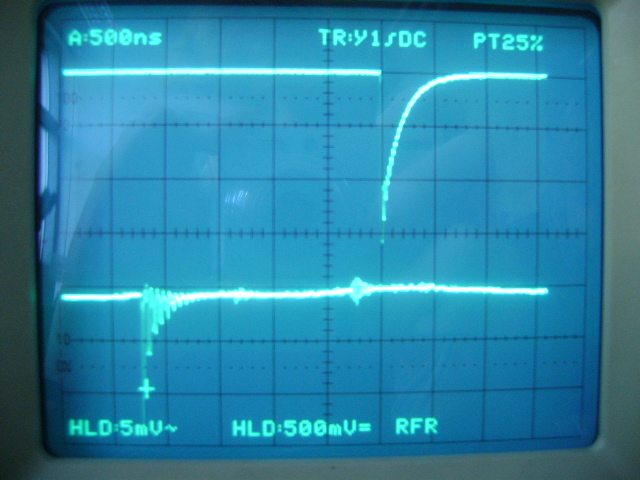
\includegraphics[width = \textwidth]{messergebnisse/5.JPG}
\end{minipage}
\begin{minipage}{0.6\textwidth}
\centering \begin{tabular}{l l}
Verstärkung & 1000\\
Shaping Time & 0.5 $\mu s$\\
Tiefe des Signals & 1.6 V\\
Breite des Signals & 0.7 $\mu s$
\end{tabular}
\end{minipage}
\end{figure}

Die Distanz zwischen beiden Peaks ist hier etwa 2.2 $\mu s$. Durch Einstellen des Delays kann man diese ändern. Wir haben uns den Einfluss klar gemacht und folgende Werte gemessen:\\

\begin{center}
\begin{tabular}{l c c c c}
Delay & 0.12 & 3.0 & 7.4 & 10.0\\
$\Delta t / \mu s$ & 2.25 & 2.6 & 3.0 & 3.2
\end{tabular}
\end{center}

Die Erhöhung des Lower Levels hat dazu geführt, dass wir seltener ein Signal erhalten haben. Ist der Lower Level zu hoch, so erhält man kein Signal mehr. Ebenso erhält man kein Signal mehr, wenn man den Upper Level zu niedrig einstellt. Ist er zu hoch, so flackert das Signal.\\

Der positive Ausgang des Einkanalanalysators hat anstatt eines negativen Peaks, wie beim negativen Ausgang, einen Kasten mit positiver Amplitude herausgegeben. Bei einer Verstärkung von 1000 und einer Shaping Time von 0.5 $\mu s$ hatte der Kasten eine Amplitude von 6 V und eine Breite von 0.5 $\mu s$. Die Einstellungen, wie z.B. Verstärkung, Delay und Shaping Time hatten den gleichen Einfluss auf das positive wie auf das negative Signal.\\

Im Unterschied zum Plastikszintillator ist das Signal des NaI-Szintillators viel stärker. Die Shaping Time kann auch viel freier gewählt werden, ohne dass das Signal zu flackern beginnt. Z.B. haben wir bei einer Verstärkung von 30 und einer Shaping Time von 10 $\mu s$ ein Signal am unipolaren Ausgang mit einer Amplitude von etwa 7 V und einer Peak to Peak-Länge von 30$\mu s$ erhalten. Das Signal sieht anders aus als beim Plastikszintillator, nämlich hat man hauptsächlich einen großen, positiven Peak und dann noch einen kleinen negativen, der etwa 10 mal kleiner ist. Beim bipolaren Ausgang erhält man ein Signal mit 2 gleich großen Peaks und mit der oben genannten Einstellung erhielten wir die Peak to Peak-Amplitude von 12 V und eine Zeitdifferenz von 22 $\mu s$ zwischen den Peaks.

\subsection{Blockschaltbild des Versuchs}

\begin{figure}[H]
\centering 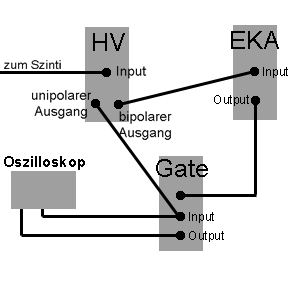
\includegraphics[width = 0.6\textwidth]{Bilder/Schema.png}
\caption{Blockschaltbild des Versuchs}
\end{figure}

\subsection{Energieeichung des MCA}

Wir haben für die Messungen den NaI-Szintillator benutzt. Zur Energieeichung des Vielkanalanalysators haben wir die Spektren von 3 Proben aufgenommen, nämlich $^{22}Na$, $^{60}Co$ und $^{152}Eu$. Alle Messungen wurden mit der Verstärkung 20 und der Shaping Time 2 $\mu s$ aufgenommen.

Die bekannten Peaks der Spektren der 3 Proben wurden mit einer Gaußkurve gefittet. Aus diesen Peaks und den theoretischen Werten dieser Peaks, können wir nun die Energie-Kanal-Abhängigkeit ausrechnen. Die aus den Graphen ermittelten Werte sind folgende:\\

\begin{center}
\begin{tabular}{| l | c | c | c | c | c | c |} \hline
Präparat & $^{22}Na$ & $^{22}Na$ & $^{60}Co$ & $^{60}Co$ & $^{152}Eu$ & $^{152}Eu$\\ \hline
Energie / keV (theoretisch) & 511 & 1274 & 1173 & 1332 & 122 & 344\\ \hline
Kanal & 146.8 & 354.1 & 326.1 & 369.3 & 38.1 & 100.4\\ \hline
$\chi^2$/ndf & 1.24 & 1.70 & 0.82 & 1.14 & 65.40 & 5.09\\ \hline
\end{tabular}
\end{center}

Die theoretische Werte wurden aus der Staatsexamensarbeit entnommen. Den Fehler auf den Kanal schätzen wir 3. Auf den theoretischen Wert der Energie nehmen wir keinen Fehler an.

\begin{figure}[H]
\centering 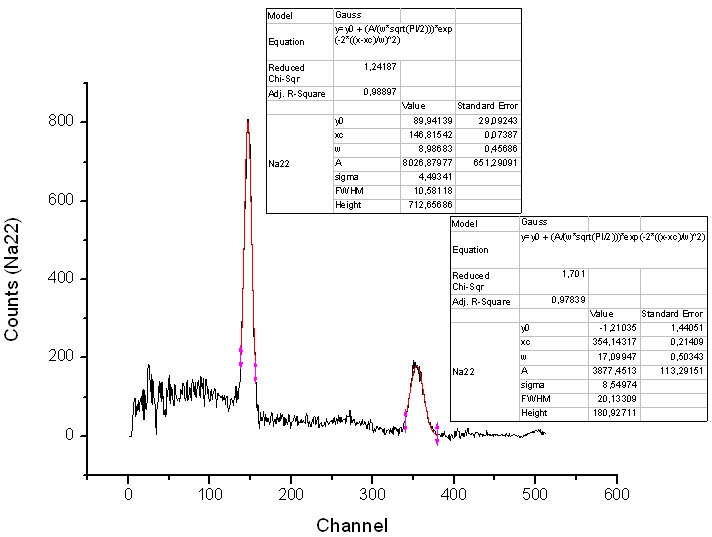
\includegraphics[width = 0.85\textwidth]{auswertung/Na22.png}
\caption{$^{22}Na$}
\end{figure}

\begin{figure}[H]
\centering 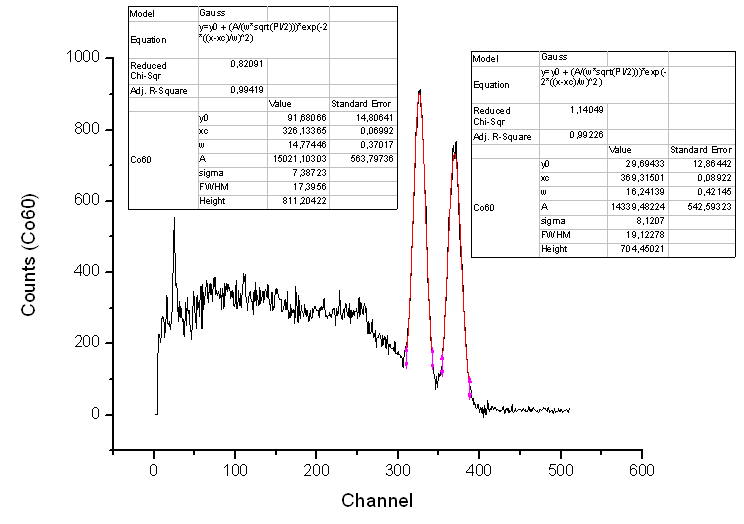
\includegraphics[width = 0.85\textwidth]{auswertung/Co60.png}
\caption{$^{60}Co$}
\end{figure}

\begin{figure}[H]
\centering 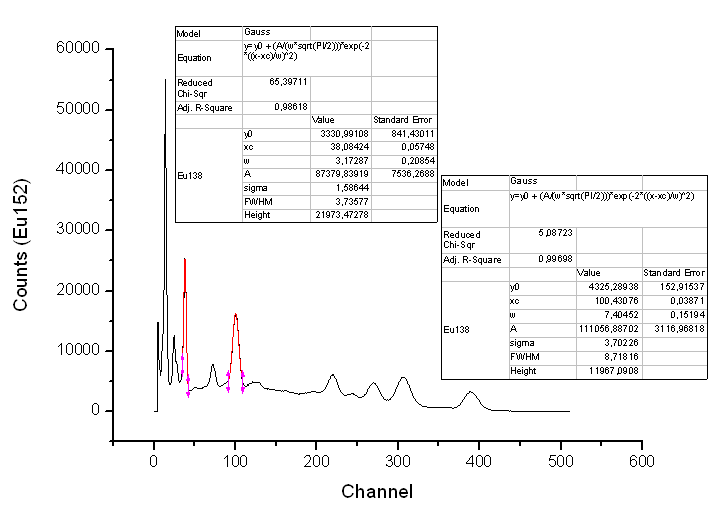
\includegraphics[width = 0.85\textwidth]{auswertung/Eu152.png}
\caption{$^{152}Eu$}
\end{figure}


In dem wir den Kanal gegen die Energie auftragen, können wir per linearen Fit die Abhängigkeit dieser beiden Größen berechnen (siehe hierzu den Anhang). Als Steigung erhalten wir:

$$ b = (3.662 \pm 0.011) $$

und als Achsenabschnitt

$$ a = (-21.91 \pm 2.76) keV $$

Somit ist die Umrechnung vom Kanal K in Energie E:

$$ \boxed{E = bK + a = 3.662\cdot K - 21.91} $$ 
mit dem Fehler
$$ s_E = \sqrt{K^2s_b^2 + b^2s_k^2 + s_a^2} = \sqrt{0.000114\cdot K^2 + 128.30} $$

\subsection{Auswertung des Thoriums}

\begin{figure}[H]
\centering 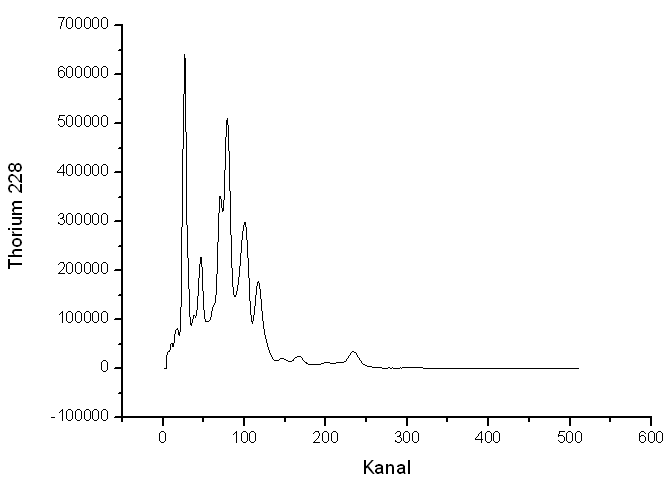
\includegraphics[width = \textwidth]{auswertung/Thoriumganz.png}
\caption{Untergrundkorrigiertes Spektum von $^{228}Th$}
\end{figure}

Die Thoriumprobe wurde 55530.307 s lang gemessen. Der Untergrund wurde hochgerechnet und dann vom Spektrum abgezogen. Wir erhalten das oben dargestellte Spektrum. Zur Auswertung fitten wir wieder Gaußkurven an die Spitzen und können dann mit der oben bestimmten Energie-Kanal-Abhängigkeit die Energie der einzelnen Peaks ausrechnen und dann interpretieren.

Wir erhalten folgende Kanäle und daraus folgende Energien:

\begin{center}
\begin{tabular}{| c | r | r | c |} \hline
Peak & Kanal & Energie E & $s_E$\\ \hline
1 & 26.74 & 76.0 & 11.3\\
2 & 46.30 & 147.6 & 11.3\\
3 & 70.91 & 237.7 & 11.4\\
4 & 78.67 & 266.1 & 11.4\\
5 & 99.18 & 341.2 & 11.4\\
6 & 117.04 & 406.6 & 11.4\\
7 & 146.33 & 513.9 & 11.4\\
8 & 166.23 & 586.8 & 11.5\\
9 & 233.66 & 833.7 & 11.6\\ \hline
\end{tabular}
\end{center}

Einen erwarteten 10. Peak von etwa 2.6 MeV konnten wir nicht sehen, da wir die Verstärkung so eingestellt haben, dass der Maximalwert für die Energie bei Kanal 512 nur 1.85 MeV war. Hier eine übersicht der gefitteten Peaks:

\begin{figure}[H]
\centering 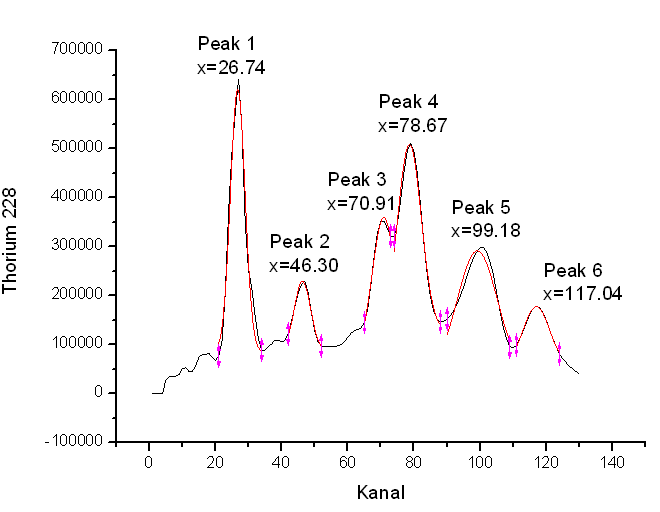
\includegraphics[width = \textwidth]{auswertung/Th1.png}
\caption{Erster Teil des $^{228}Th$-Spektrums}
\end{figure}

\begin{figure}[H]
\centering 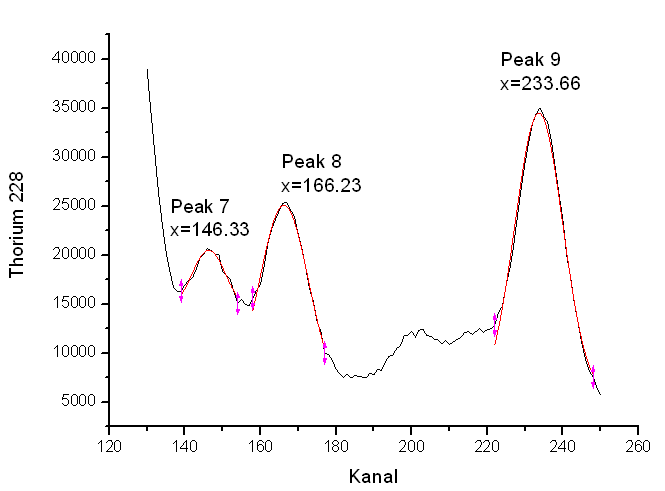
\includegraphics[width = \textwidth]{auswertung/Th2.png}
\caption{Zweiter Teil des $^{228}Th$-Spektrums}
\end{figure}

\subsection{Interpretation der Peaks des Thorium-228-Spektrums}

\begin{center}
\begin{tabular}{| c | r | c | p{6cm} | c |} \hline
Peak & E / keV & $E_{theo}$ / keV & Interpretation &St-Abw. \\ \hline
1 & 76.0 $\pm$ 11.3  & 84.37 & $^{228}Th \rightarrow ^{224}Ra$, wahrscheinlichster Übergang & 1 \\
2 & 147.6 $\pm$ 11.3 & 131.6 und 166.4 & $^{228}Th \rightarrow ^{224}Ra$, Überlagerung der beiden Peaks der theoretischen Energien & jeweils 2\\
3 & 237.7 $\pm$ 11.4 & 216.0 & $^{228}Th \rightarrow ^{224}Ra$ & 2\\
4 & 266.1 $\pm$ 11.4 & 241.0 und 238.6 & $^{224}Ra \rightarrow ^{220}Rn, \text{\ \ sowie \ \ } ^{212}Pb \rightarrow ^{212}Bi$, beide Peaks sind überlagert & jeweils 3\\
5 & 341.2 $\pm$ 11.4 & 300.1 & $^{212}Pb \rightarrow ^{212}Bi$ & 4\\
6 & 406.6 $\pm$ 11.4 & 453.0 & $^{212}Bi \rightarrow ^{208}Tl$ & 4\\
7 & 513.9 $\pm$ 11.4 & 510.8 & $^{208}Tl \rightarrow ^{208}Pb$ & 1\\
8 & 586.8 $\pm$ 11.5 & 583.2 & $^{208}Tl \rightarrow ^{208}Pb$ & 1\\
9 & 833.7 $\pm$ 11.6 & 804.9 & $^{216}Po \rightarrow ^{212}Pb$ & 3\\ \hline
\end{tabular}
\end{center}

\emph{St-Abw.} gibt die Anzahl der Standardabweichungen an, in denen der theoretische Wert der Energie von dem gemessenen liegt. Unsere Werte liegen also alle in einem guten Bereich, nahe genug an den erwarteten Werten. Angegeben bei der Interpretation ist immer der Zerfall des Mutterkerns in den Tochterkern, welcher dann ein $\gamma$-Quant der genannten Energie emittiert, um in den Grundzustand über zu gehen.


\subsection{Interpretation der auftretenden intensiven Linie des Untergrunds}

\begin{figure}[H]
\centering 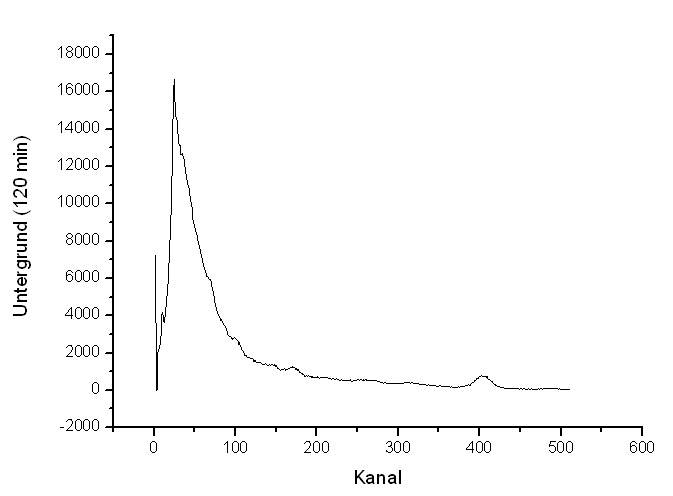
\includegraphics[width = \textwidth]{auswertung/UG1.png}
\caption{Der gemessene Untergrund (120 min)}
\end{figure}

Wir untersuchen den etwas intensiveren Peak bei Kanal 400. Nach einem Gauß-Fit erhalten wir einen Wert für den Kanal von 403.58. Für die Energie folgt somit:

$$E = (1456.0 \pm 12.2) keV $$

Wir interpretieren dies als ein Kalium-40-Peak ($E_{theo} = 1460.8$, 1 Standard-Abweichung), da der Gauß-Fit sehr dicht an dem Wert liegt, und da Kalium in der Umgebung vorkommt.

\begin{figure}[H]
\centering 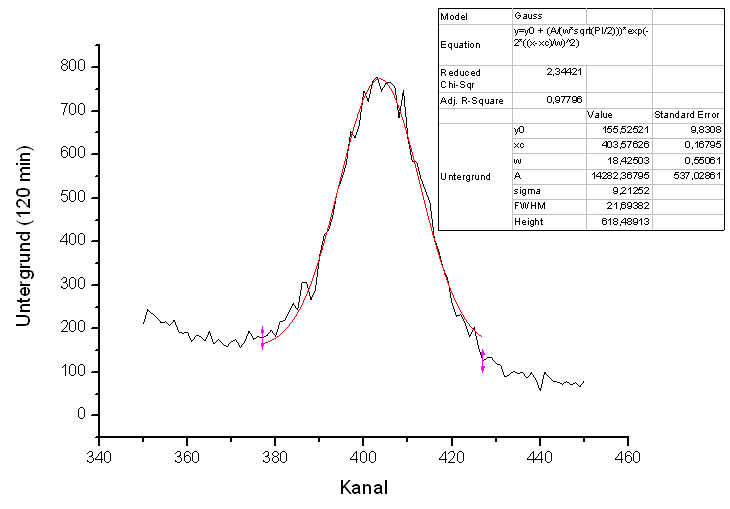
\includegraphics[width = \textwidth]{auswertung/UG2.png}
\caption{Zoom auf Kanäle 350-450 des Untergrunds}
\end{figure}

\subsection{Winkelverteilung der $^{22}Na$ Vernichtungsphotonen}

Bevor wir mit der Messung begonnen haben wir die Levels (upper und lower level) angepasst, so dass nur die $\gamma$-Quanten gemessen werden, die eine Energie von 511 keV haben. Außerdem mussten anhand des Delays beide Szintillatoren so eingestellt werden, dass sie zeitgleiche Signale herausgeben, damit die Koinzidenzen auch tatsächlich gemessen werden konnten.\\

Zur Koinzidenzmessung haben wir dann den Plastikszintillator gegenüber vom NaI-Szintillator gedreht, und zwar um einen Winkel von 90$^\circ$ bis 200$^\circ$. Es wurden jedes mal 120 s gemessen. Nach den Messungen haben wir noch eine Messung ohne Probe gemacht, bei der wir 5 counts erhalten haben. Dieser Untergrund (zufällige Koinzidenzen) wurde von den ermittelten Werten abgezogen.\\

Der Fehler auf die Counts (Fehlerbalken) berechnet sich durch $s_N = \sqrt{N}$. Den Fehler auf den Einzelwert haben wir mit $s_\alpha = 0.5^\circ$ abgeschätzt.

\begin{figure}[H]
\centering 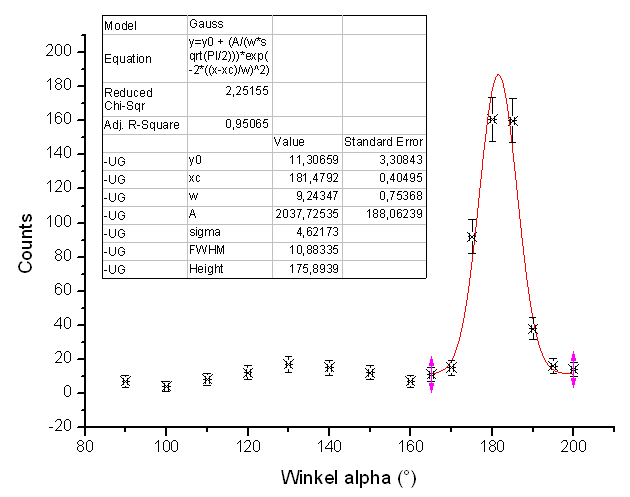
\includegraphics[width = \textwidth]{auswertung/Winkel.png}
\caption{Winkelverteilung der Vernichtungsphotonen}
\end{figure}

Das Maximum liegt also bei
$$\alpha = (181.48 \pm 0.40)^\circ$$
Wir konnten somit die theoretische Vorhersage von 180$^\circ$ bestätigen. Dieser Wert liegt in der 4. Standardabweichung. Wir gehen bei der kleinen Abweichung eher von einem systematischen Fehler aus, welcher jedoch sehr klein ist.

Messtabelle (mit Untergrundkorrektur)

\begin{center}
\begin{tabular}{c c c c c c c c}
90$^\circ$ & 100$^\circ$ & 110$^\circ$ & 120$^\circ$ & 130$^\circ$ & 140$^\circ$ & 150$^\circ$ & 160$^\circ$\\ \hline
7 & 4 & 8 & 12 & 17 & 15 & 12 & 7 \\
& & & & & & & \\
165$^\circ$ & 170$^\circ$ & 175$^\circ$ & 180$^\circ$ & 185$^\circ$ & 190$^\circ$ & 195$^\circ$ & 200$^\circ$\\ \hline
11 & 15 & 92 & 161 & 160 & 38 & 16 & 14\\
\end{tabular}
\end{center}


























\clearpage
\section{Zusammenfassung}

Im ersten Teil des Versuchs haben wir das Magnetfeld des Permanentmagneten mit einer Hallsonde vermessen, um herauszufinden, an welchen Stellen das Magnetfeld homogen ist, und wie stark das Feld an dieser Stelle ist. Die Ermittlung der Homogenität haben wir bei den weiteren Messungen benutzt, die Magnetfeldstärke beträgt:

$$ \boxed{B = (434.1 \pm 4.5)\ mT} $$

Dann haben wir versucht die Resonanzfrequenz der 3 vorliegenden Proben zu messen, indem wir die Frequenz so verändert haben, dass die Absorptionslinien äquidistant waren. Diese Frequenz wurde dann gemessen und daraus der Landé-Faktor $g$ und das gyromagnetische Verhältnis $\gamma$ berechnet:


\begin{center}
\begin{tabular}{| l | c | c | c | c |} \hline
Probe & $\nu_r$ / MHz & $g$ & $\sigma(g)$ & $\gamma\ / MHz\cdot T^{-1}$\\ \hline
Glykol & $18.184 \pm 0.050$ & $5.495 \pm 0.059$ & 2 & $263.2 \pm 2.8$ \\
Wasserstoff &$18.180 \pm 0.002$ & $ 5.494 \pm 0.057 $ & 2 & $263.2 \pm 2.7$ \\
Teflon & $17.114 \pm 0.002$ &  $5.172 \pm 0.054$ & 2 & $247.7 \pm 2.6$\\ \hline
\end{tabular}
\end{center}

Für die Teflonprobe haben wir dann noch das kernmagnetische Moment $\mu_K$ berechnet, indem wir den Wert für $g$ als gegeben annahmen. Wir erhielten den Wert:

$$\boxed{\mu_K = (4.968 \pm 0.052)\cdot 10^{-27} J/T} $$

Der theoretische Wert liegt in der 2.Standard-Abweichung von diesem Wert.

Mithilfe der Wasserstoffprobe haben wir eine zweite Messung der Homogenität des Magnetfeldes durchgeführt und einen leichte lineare Zunahme der Magnetfeldstärke in x-Richtung bzw. eine lineare Abnahme in y-Richtung auf dem vorhin ermittelten Plateau feststellen können.

Im letzten Teil des Versuchs haben wir anhand des Lock-In-Verfahrens durch einen linearen Fit noch ein Mal die Resonanzfrequenz der Wasserstoffprobe gemessen und erhielten:

$$\boxed{\nu_r = (18.1893 \pm 0.0019)\ MHz}$$

Dieser Wert liegt sehr dicht an der vorher ermittelten Resonanzfrequenz (0.051\% Abweichung). Weiterhin konnten wir mit dieser Resonanzfrequenz auch den Landé-Faktor berechen und erhielten
$$ g = 5.497 \pm 0.057 $$ 

welcher in der 2. Standardabweichung des Literaturwerts $g_{lit,H} = 5.5856$ liegt.
\section{Anhang}

\begin{appendix}
 
\end{appendix}


\clearpage

%\bibliographystyle{alphadin} 
%\bibliography{bib}


\end{document}
